\documentclass[twocolumn]{article}
\usepackage[utf8]{inputenc}
\usepackage{natbib}
\usepackage{graphicx, caption}
\usepackage{authblk}
\usepackage{textcomp}
\usepackage[usenames,dvipsnames]{xcolor}
\usepackage{amsmath}

\usepackage{multicol}
\usepackage[textwidth=492.982pt, top=2cm, bottom=2cm]{geometry}

\newcommand*{\cyril}{\textcolor{ForestGreen}}

\graphicspath{{./figures}{./}}

\title{Macroscopic description of particle-laden gravity currents: overall perspectives}
\author{Gadal C., Schneider J., Bonamy C., Chauchat J., Dossmann Y., Kiesgen de Richter S., Mercier M., Naaim F., Rastello M., Lacaze L.}
\date{{\it\color{red}Deadline: May 31$^{st}$}}

\begin{document}

\twocolumn[

	\maketitle

	\begin{abstract}
		Particle-laden gravity currents (PLGCs) are driven by a mass difference between an heavy fluid-particle mixture and a lighter ambient liquid.
		We focus our attention on finite volume current, generated here by lock-release device over a controlled constant slope bottom at the laboratory scale.
		The main objective of the present chapter is to provide a comprehensive flow regime associated with the relevant dimensionless parameters which characterize the current at the macroscopic scale, i.e. average over the current depth.

	\end{abstract}

	\vspace{0.3cm}
	{\it \color{red}REMINDER: Word limit of about 10,000 per article, plus 7 figures.}\\
	\vspace{0.3cm}
]

\section{Introduction}
\label{sec:intro}

\cyril{
	\begin{itemize}
		\item définir $U_{0} = \sqrt{g' H_{0}}$ dans l'intro déjà ?
		\item inclure le $\cos\alpha$ dans cete definition directement ? $U_{0} = \sqrt{g' H_{0} \cos\alpha}$
	\end{itemize}
}

\subsection{Finite volume density currents}

Density currents have been widely considered at the laboratory scale for their ubiquitous occurrence in geophysical flows \citep{Hopfinger1983,Simpson1999,Dufek2016}. As they are mostly associated with unsteady and non-uniform dynamics in nature, the lock-release device appeared to be a popular canonical configuration to mimic their behaviour at the laboratory scale \citep{Hacker1996,Shin2004,Nogueira2014}. In particular, studies often focused on characterising the front dynamics and the front shape as a macroscopic description of the underlying complex dynamics \citep{Rottman1983,Marino2005,Hogg2006}.

The basic approach to describe a lock-release evolution is built upon characteristics solutions of the hyperbolic shallow water equations for an inviscid dense liquid of density $\rho_c$ slumping on a horizontal bottom under an inertialess and weightless ambient fluid. Among others, this specifically allows quantifying a most obvious scaling analysis solution reading for the front velocity $U_c$ reading
\begin{equation}
	U_c\propto \sqrt{gH_0},
\end{equation}
with $g$ the gravity and $H_0$ the initial height of the fluid volume being released. The method of characteristics suggests a coefficient of proportionality of exactly $2$ between velocities $U_c$ and $\sqrt{gH_0}$. An extension towards a weighted ambient fluid of density $\rho_a$ shall lead to
\begin{equation}
	U_c\propto \sqrt{g'H_0},\quad\mbox{with}\quad g'=\frac{\rho_c-\rho_a}{\rho_c}g.
	\label{eq:solUc}
\end{equation}
However, the coefficient of proportionality now requires slightly more attention as it is clearly found smaller than $2$ in experiments or simulations \citep{??}. The main reason is that most density currents are characterized by a small density ratio between current and ambient, making the assumption of inertialess ambient fluid unlikely.
Knowledge of the front velocity then requires a local description of the flow close to the front, which in turn adds the characteristic height of the ambient as a required control parameter, as suggested by \citet{Benjamin1968}.
In the case of lock-release configuration, it would suggest an influence of the ratio between reservoir height $H_0$ and ambient height $H$.
Nevertheless, obtained results allow linking the front velocity to the height of the current close to the front, which is a priori unknown in a lock-release device, i.e. the front relation includes two unknowns \citep{Benjamin1968}. Models have been proposed to circumvent this issue, leading for instance to a coefficient of proportionality $0.5 (\rho_c/\rho_a)^{1/2}(H/H_0)^{1/3}$ between the two velocities in \eqref{eq:solUc} \citep{Huppert1980}. The latter coefficient is relevant for not two deep ambient $H$ compared to the reservoir height $H_0$, which is actually the case in most experiments. Most configurations correspond to $H=H_0$, which would lead to a value of $0.5$. Even if several experiments and numerical simulations confirm such a value around $0.5(\rho_c/\rho_a)^{1/2}$, its exact value remains still unclear, and probably dependent on several physical processes. In particular, these velocities relationships during the slumping regime are based on negligible dissipation during this regime, which shall be violated in some cases, as significant mixing with the ambient at the miscible interface,  settling particles, etc.

The slumping regime ends when either the rarefaction wave associated with finite volume or dissipation induced by bottom friction and entrainment at the miscible interface, overcomes the current dynamics \citep{???}.
From dimensional analysis, a transition length scale $X_{\rm t}$ towards these regimes would lead, respectively, to
\begin{equation}
	\label{eq:Xt_inertial}
	\displaystyle    X_{\rm t}=  \frac{2L_0 }{\sqrt{g'H_0}/U_c - 1},
\end{equation}
\begin{equation}
	\label{eq:Xt_drag}
	\displaystyle    X_{\rm t}=H_0  \frac{g'H_0}{C_dU_c^2},
\end{equation}
with $C_d$ some drag coefficient induced by friction at the bottom and by entrainment at the interface. This would give with the previous estimation of the velocity ratio $0.5(\rho_c/\rho_a)^{1/2}$ during the slumping regime, respectively,
$X_{\rm t}=2L_0/[2(\rho_a/\rho_c)^{1/2}-1]$ \textcolor{blue}{A voir? } and $X_{\rm t}=[4(\rho_a/\rho_c)H_0]/C_d$.
%\begin{equation}
%\displaystyle    X_{\rm t}=2L_0/[2(\rho_a/\rho_c)^{1/2}-1],
%\end{equation}
Details of such transitions actually depend on the complex details of the flow and drag induced by the current intruding the ambient and the friction at the bottom. These transitions then become case-dependent and required parametrization. For instance, following experiments of \cite{Rottman1983}, it was found that???
%Moreover, another transition has also been reported in the literature, referred to as the buoyancy-inertia regime \citep{Hoult1972}. Yet, this regime is hardly visible, probably due to the succession of different temporal law evolution of the front from the constant slumping regime towards the decelerating viscous regime, and can be disregarded for the purpose of the present study \citep{Huppert1980}. 

%The slumping regime ends when either the rarefaction wave associated with finite volume or dissipation induced by bottom friction and entrainment at the miscible interface, overcome the current dynamics \citep{???}. 
%By dimensional analysis, they lead to transition length scale $X_{\rm t}$, respectively
%\begin{equation}
%\displaystyle    X_{\rm t}= 2L_0  \frac{1}{\sqrt{g'H_0}/U_c - 1},
%\end{equation}
%\begin{equation}
%\displaystyle    X_{\rm t}=H_0  \frac{g'H_0}{C_dU_c^2},
%\end{equation}
%with $C_d$ some drag coefficient induced by friction at the bottom and by entrainment at the interface. This would give with the previous estimation of the velocity ratio $0.5$ during the slumping regime, respectively 
%\begin{equation}
%\displaystyle    X_{\rm t}=2L_0,
%\end{equation}
%\begin{equation}
%\displaystyle    X_{\rm t}=\frac{4H_0}{C_d}.
%\end{equation}

Constant bottom slope $\alpha$, often relevant to characterise the main process of natural flow over topography, adds complexity to this front analysis. In particular, including a bottom slope into the previous slumping regime is not obvious as it would suggest a constant acceleration of the flow, at least until balanced by friction at both the interface and the bottom. Yet, constant regime flows are observed at early stages in experiments and simulations prior to such balance \citep{Birman2007,???}. It has been shown that the reason for that is the relatively long time or length scales over which acceleration imposed by the slope overcome flow induced by the lock-release pressure gradient. A way to highlight that is a simple dimensional balance between slope and pressure gradient. This can be written as
%\begin{equation}
%\displaystyle    (\rho_c - \rho_a)g \sin{(\alpha)} %= \frac{(\rho_c - \rho_a)g \cos{(\alpha)}H_0}{X_{\rm t}},
%\end{equation}
\begin{equation}
	\label{eq:Xt_slope}
	X_{\rm t}=H_0\tan^{-1}{(\alpha)}.
\end{equation}
where $X_{\rm t}$ corresponds to the length scale over which slope effect and pressure gradient balance, and can be seen as a transition length scale over which slope drives the current until reaching the next equilibrium between slope and friction.
Nevertheless, the slope can affect the specific relationship \eqref{eq:solUc} linking the velocity scales during the slumping regime \citep{Birman2007,???}. Such a relationship still needs to be clarified.

%%%%%%Figure 1
\begin{figure*}[ht!]
	\centering
	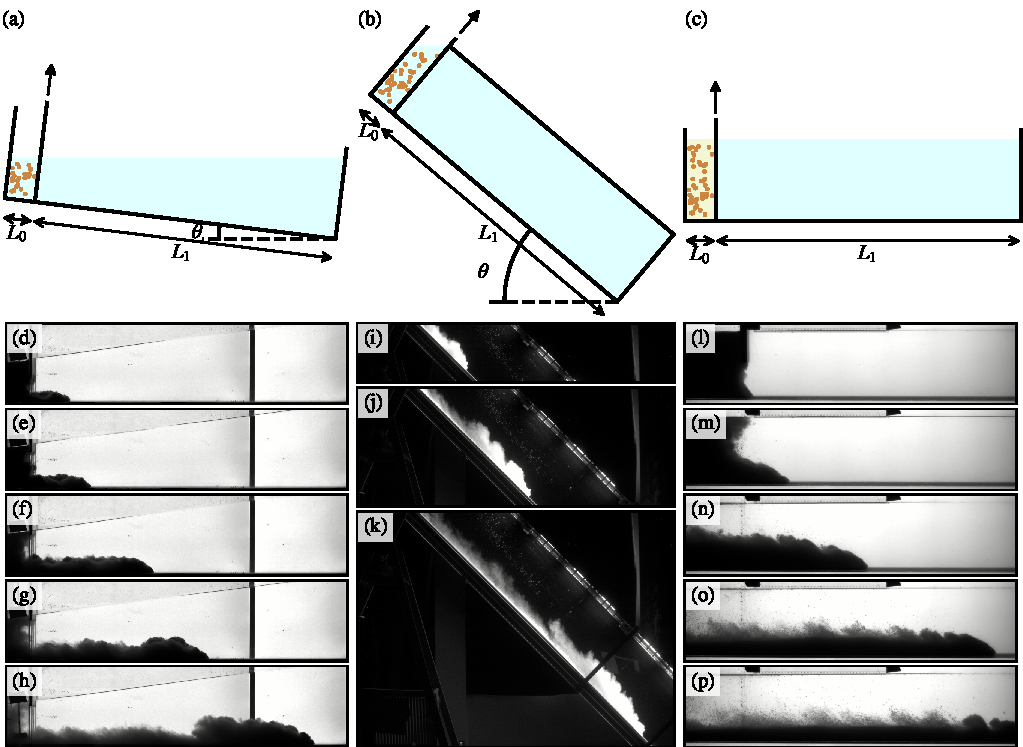
\includegraphics{figure1.pdf}
	\caption{\textbf{Experimental set-ups used in this study.} (a--c) Sketches of the three experimental set-ups. Below are shown snapshots of corresponding experimental images. (d--h) Set-up 1, $\alpha = 7^\circ$, $\phi \sim 3~\%$, $\mathcal{S}t=$ (i--k) Set-up 2, $\alpha = $, $\phi \sim $, $\mathcal{S}t=$ (l--p) Set-up 3, $\alpha = $, $\phi \sim 55\%$, $\mathcal{S}t=$.}
	\label{fig:fig1}
\end{figure*}
%%%%%%%%

\subsection{Particle-Laden Gravity Currents}

Particle-Laden Gravity Currents (PLGCs) refer to as gravity currents, or density currents, are driven by a mass difference between a heavy fluid-particle mixture and a lighter ambient liquid \citep{Hopfinger1983,Middleton1993,Kneller2000,Meiburg2010,wells2021}. Different subclasses of PLGCS can be distinguished depending on the relative density of the different phases constituting the system; i.e. the particle phase, the carrier fluid phase and the ambient fluid phase. In the following, we will focus on two of them, characterized by only two distinct densities. At one end, the carrier phase and ambient phase are the same fluid and particles are heavier. This is the most commonly studied subclass of PLGCs, usually referred to as turbidity currents. At the other end, PLGCs can also be induced by a neutrally-buoyant fluid-particle mixture flowing into a lighter ambient fluid. A major difference between PLGCs and compositional currents is therefore the existence of typical length and time scales associated with the particle dynamics.
%At one end, the own settling velocity of heavy particle only allow the existence of these gravity currents on finite time scale and finite length scale.
Nevertheless, the prediction of these finite scales is difficult as it shall strongly depends on the interaction between particle dynamics and the local turbulence of the carrying fluid and/or ambient fluid at the upper interface, which modifies entrainment and associated dissipation. In turn, this can modify the macroscopic behaviour of the current, as for instance the dynamics of the front. Accordingly, their dynamics shall be controlled by several dimensionless parameters leading to a wide variety of flow regimes. In particular, beyond the slope $\alpha$, the dimensionless density difference between the current and the ambient $At$ and the ratio between available inertia and dissipation, say a Reynolds number $Re$, as usually introduced as a control parameter for any density currents, the initial solid fraction of particles $\phi$ and a dimensionless settling velocity $St$ have now to be considered as potentially affecting flow regimes. It shall be noted that in some specific situations, some of these dimensionless parameters could be linked, for instance, $\phi$ and $At$ for heavy particles in a single-phase liquid for the carrying and ambient fluids.

Following the balance scaling as done far, a transition between the equivalent slumping regime as described for gravity current and deposition of particle. Instead of dynamical scaling as done previously, here a kinematic scaling is obtained as the balancing time scale of current propagation and time scale of particle settling. This leads to
\begin{equation}
	\label{eq:Xt_settling}
	X_{\rm t}=H_0\frac{U_c}{V_s},
\end{equation}
in which $V_S$ is the settling velocity of the solid particles within the PLGCs. Of course, such transition disappears for the neutrally-buoyant situation described previously.
Again, such an approach only gives a scaling of transition, but the influence of the particle dynamics prior to such transition remains unclear.
Overall, the specific ratio between velocities in \eqref{eq:solUc} in the slumping inertial regime remains to clarify varying the influence of the mechanisms discussed so far.

\section{Dimensional analysis at the macroscopic scale of the current}
\label{sec:dimensionlessmap}

%%%%%%Figure 2  
\begin{figure}
	\centering
	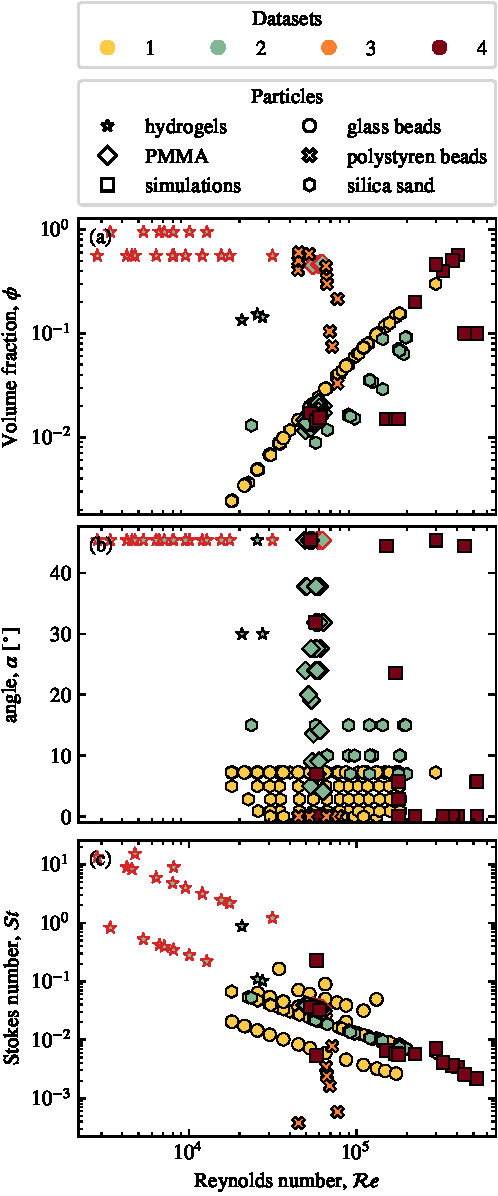
\includegraphics{figure2.pdf}
	\caption{\textbf{Explored parameter space.} Each symbol corresponds to a single experimental run.}
	\label{fig:fig2}
\end{figure}
%%%%%%%%%%

Here, the dimensionless parameters are based on a characteristic length $L_0$ and a characteristic velocity $U_0=\sqrt{g' H_0}$ where $L_0$ and $H_0$ are the horizontal length and depth of the initial container, respectively, $g'$ is the modified gravity $ g \cos{\alpha}(\rho_m-\rho_a)/\rho_m$ with $\rho_m$ the current mixture density (analogous to $\rho_c$ as for current in \eqref{eq:solUc}) and $\rho_a$ the current density and ambient fluid density respectively. Note that $g'$ is slightly different from the definition in section \ref{sec:intro}. Here $g'$ is written with the ambient density at the denominator, i.e. as to include the influence of density ratio on front velocity as discussed in section \ref{sec:intro}. The mixture density can be quantified as $\rho_m = \phi \rho_p+(1-\phi)\rho_f$ with $\rho_p$ the particles density and $\rho_f$ the fluid phase density initially in the current. In the set of experiments presented here $\rho_f\le \rho_a$. The velocity scale $U_0$ corresponds to an idealized transfer of initial potential energy to kinetic energy along the slope, i.e. a collapse of the initial column. Accordingly,
\begin{equation}
	\displaystyle a =\frac{H_0}{L_0},
\end{equation}
\begin{equation}
	\displaystyle Re = \frac{U_0 H_0\rho_m}{\eta_f},
\end{equation}
\begin{equation}
	\displaystyle At = \frac{\rho_m-\rho_a}{\rho_a},
\end{equation}
%\textcolor{blue}{Rem: avant on avait $(\rho_m-\rho_a)/\rho_a$. qu est ce que cela change.}
\begin{equation}
	\displaystyle St = \frac{V_s}{U_0},
\end{equation}
with $\eta_f$ the interstitial fluid viscosity and $V_s$ the Stokes settling velocity in the interstitial fluid phase labelled $f$. Note that $At$ usually intervenes only in the modified gravity $g'$ for Boussinesq currents, which is mostly the case for density currents \citep{Bonometti2011,???}

Then, the dynamics of the current is characterised by several dimensionless variables. The most common one to be analysed in gravity-driven avalanches is the dimensionless front velocity, also referred to as the Froude number,
\begin{equation}
	\displaystyle \mathcal{F}r =\frac{U_c}{U_0},
\end{equation}
where $U_c$ is the front velocity of the current. Note that $U_c$ is time-dependent, and so is $\mathcal{F}r$, i.e. that $\mathcal{F}r$ as defined here is not a control parameter. (The Froude number which would be defined as a control parameter for a lock-release configuration would be $Fr\equiv 1$, and is thus not relevant to predict the flow dynamics.)

\section{Methods}

\subsection{Experimental setups}
Even if the dynamics of PLGCs is associated with several complex processes, a general consequence is observed in the front dynamics, often referred to as the $\mathcal{F}r$ number, and the front shape. Then prediction of the different flow regimes associated with PLGCs shall be entirely included in these observables. In order to characterize the different flow regimes for PLGCs induced by a finite volume of material initially at ``rest'', 3 dam-break-type devices have been used to cover a wide range of control parameters, These experimental devices are supplemented with Euler-Euler numerical simulations to confirm the relevance of such flow regime description to characterize the dynamics of PLGCs.

All setups are based on the same typical lock-release design (see figure~\ref{fig:fig1}). In particular, a tank of length $L_0+L_1$ along the streamwise direction $x$, width $W_0$ and height $H_0$, is separated by a sluice gate at a distance $L_0$ from one end along $x$, allowing to distinguish an initial reservoir in which the particle-laden mixture is prepared from the ambient fluid. The sluice gate is lifted up manually at $t=0$ to initiate the gravity current.

\paragraph{Set-up 1}

The first set-up (figure~\ref{fig:fig1}(a)) has $L_0+L_1=150~\textup{cm}$ with $L_0 = 10~\textrm{cm}$. The upper boundary is a free surface and the tank can be tilted at an angle $\alpha=[0^\circ,7.5^\circ]$ with respect to the horizontal as shown in the 2D sketch of figure~\ref{fig:fig1}(a). The suspension is made by strongly stirring a known mass of particles within the whole water column using a chemical mixer, which is stopped just before opening the gate. In this inclined tank, $H_{0}$ is defined as the average suspension height inside the lock, equal to $20~\textrm{cm}$.
%
The current evolution is followed by a camera at 120 Hz and using a backlight as a light source.

\paragraph{Set-up 2}

Specifications of LEGI set-up

\paragraph{Set-up 3}

The third set-up (figure~\ref{fig:fig1}(c)) has $L_0+L_1=150~\textup{cm}$ with $L_0 = 20~\textrm{cm}$. The upper boundary is a free surface and the tank remains horizontal ($\alpha = 0^\circ$). Here, $H_{0}$ is between 0.2~cm and 0.3~cm depending on experiments. The current evolution is followed by a camera at 10 Hz and using a backlight as a light source.

% The suspension is made by strongly stirring a known mass of particles within the whole water column using a chemical mixer, which is stopped just before opening the gate. 

\subsection{Datasets}

On these 3 devices, $N$ experiments are presented here, complemented by $N$ numerical simulations using SedFoam (see description below). They are classified into 4 different datasets, described below.

\paragraph{Dataset 1}

The first dataset is gathered using set-up 1. A first series of experiments is made with silica sand grains of $d \sim 120~\mu\textrm{m}$ while varying the bottom slope from $0^\circ$ to $7^\circ$. Then, for $\alpha = 7^\circ$, the settling velocity is varied by using glass beads (©Silibeads) of mean diameter ranging from $60~\mu\textrm{m}$ to $250~\mu\textrm{m}$, corresponding to $V_{\rm s} \in [0.3, 3.2]~\textrm{cm}~\textrm{s}^{-1}$. A few experiments with saline water (homogeneous gravity currents) performed at this $\alpha$-value are also included in the dataset.

\paragraph{Dataset 2}

Description Dataset LEGI

\paragraph{Dataset 3}

The third dataset set is gathered using setup 3.
The experiments are performed with polystyrene beads $d \sim 1~\textrm{mm}$ in salt water (isodense gravity currents) on a slope of $0^\circ$.  The density difference between the lock and the ambient fluid is constant. Only the density varies from $~3 \%$ to $~55 \%$.

\paragraph{SedFoam}

Description Dataset SedFoam

The set of dimensionless numbers, as defined in section \ref{sec:dimensionlessmap} and covered with the different datasets, is reported in figure~\ref{fig:fig2}, with in particular (a) $\phi$, (b) $\alpha$ and (c) $St$, all as a function of $\mathcal{R}e$.
It is shown that they roughly cover the range $\phi\in[0.1\%,50\%]$, $\alpha \in [0^o,45^o]$, $St\in[10^{-3}, 10]$ and $Re\in[10^3, 10^6]$. The aspect ratio is only varied in the narrow range $a\in[2,3]$ (not shown in the figure). Its influence will not be specifically discussed in the following as it is found to be a second-order parameter in the range of parameters covered here.

\subsection{Fitting procedure and front position analysis}

%%%%%%%%%%%%%%%%%%%% Figure 3
\begin{figure*}[ht]
	\centering
	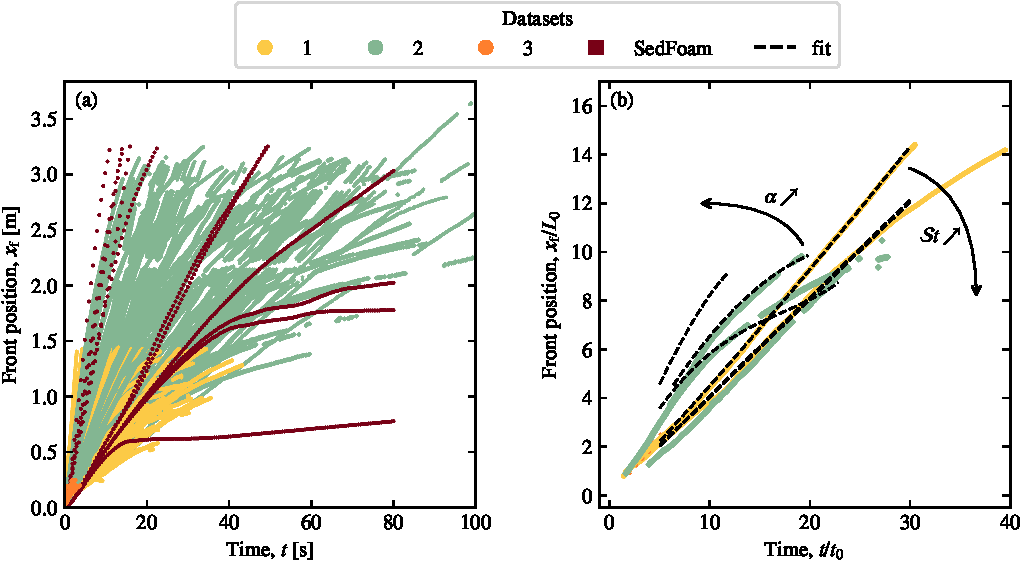
\includegraphics{figure3.pdf}
	\caption{\cyril{Panel (b) will be back to normal soon} (a) Current front position as a function of time for all experimental runs (b) Selected runs plotted in non-dimensional coordinates.}
	\label{fig:fig3}
\end{figure*}
%%%%%%%%%%%%%%%%%%%%

For each experimental/numerical run, we extract the current front position as a function of time (see Fig. \ref{fig:fig3}a). A few selected runs are shown on figure~\ref{fig:fig3}b in non-dimensional time coordinates. After a short transient acceleration phase, most currents exhibit at first a constant velocity corresponding to the so-called \emph{slumping} regime. After this, the velocity can decrease, either because of settling-induced buoyancy loss, or because the current enters the \emph{inertial} regime.

It can be qualitatively seen that increasing the bottom slope increases the slumping velocity, while increasing the Stokes number shortens the duration of the constant-velocity regime.
%
To properly quantify that, we fit all front propagation curves (except Dataset 4) with the following equation:

\begin{equation}
	\label{eq:fit_eq}
	\frac{x_{\rm f}}{L_{0}} = x_{i} + \mathcal{F}r \frac{t}{t_{0}} - \frac{\tilde{\lambda}}{2} \left(\frac{t}{t_{0}}\right)^{2},
\end{equation}
where $\mathcal{F}r$ corresponds now to the non-dimensional current velocity during the slumping regime, and $\tilde{\lambda}$ to the dissipation. The fit is performed between $t/t_{0} = 5$, to avoid the initial transient phase, and $t/t_{0} = 30$, the transition time from the slumping to the inertial regime~\citep{refs}. Note that $x_{i}$ is kept constant equal to 0 for datasets 1 and 2, but had to be left free to adjust for the SedFoam simulations \cyril{(comment this ?)}. For runs with strong dissipation ($\tilde{\lambda} > 2 {\times} 10^{-2}$), we add a quartic term to \eqref{eq:fit_eq} to improve the fit quality and obtain a better estimation of $\mathcal{F}r$ and $\tilde{\lambda}$. We checked that our results do not depend on the presence of this quartic term and that the linear and quadratic ones remain much larger.

For dataset 3, the time resolution and the experiment duration do not allow for extracting the dissipation. Therefore, we simply fit the whole available points with a linear function.

\section{Results}

\subsection{Influence of the slope on the front velocity}

The influence of the slope angle $\alpha$ on the dimensionless front velocity $\mathcal{F}r$ is presented in figure~\ref{fig:fig4}. Even if the entire set of experiments and numerical simulations are reported here, results are highlighted for $\phi < 0.45$ (see section~\ref{sec:influence_phi} for details on the influence of $\phi$).

\begin{figure*}[ht]
	\centering
	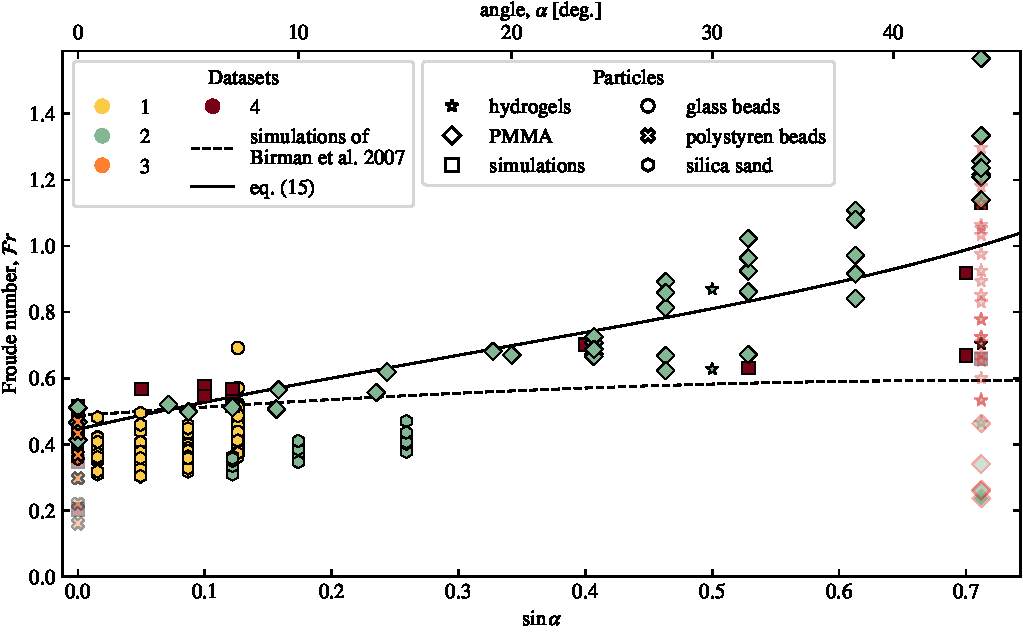
\includegraphics{figure4.pdf}
	\caption{\textbf{Influence of the bottom slope} on the current Froude number. Plain symbols correspond to $\phi < 0.45$, while transparent symbols are for $\phi \geq 0.45$ (see section~\ref{sec:influence_phi} for details on the influence of $\phi$).}
	\label{fig:fig4}
\end{figure*}

\subsection{Influence of $St$}

\begin{figure*}[ht]
	\centering
	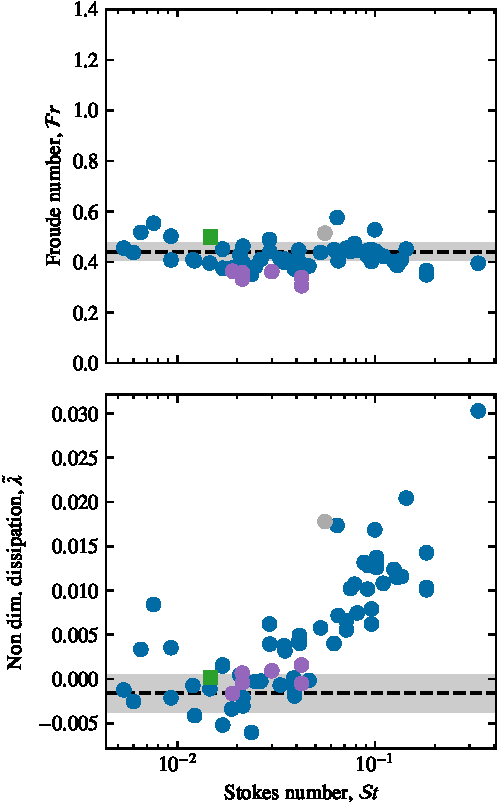
\includegraphics{figure5.pdf}
	\caption{\textbf{Influence of particle settling.} Current Froude number $\mathcal{F}r$ and attenuation $\tilde{\lambda}$ as a function of the ratio between the Stokes number and the lock aspect-ratio, for different ranges of bottom slopes. Plain symbols correspond to $\phi < 0.45$, while transparent symbols are for $\phi \geq 0.45$ (see section~\ref{sec:influence_phi} for details on the influence of $\phi$). Dotted lines mark either the average of points with $\phi < 0.45$ (a, c, e, g) or the 0 baseline (b, d, f, h). On (e, f), the dashed line indicates the average value for homogeneous saline currents ($St \equiv 0$) of dataset 1.}
	\label{fig:fig5}
\end{figure*}

In this section, we focus on the influence of settling on the current dynamics. The influence of the Stokes number $St$ on the dimensionless front velocity $\mathcal{F}r$ and attenuation $\tilde{\lambda}$ is presented in figure~\ref{fig:fig5} for different bottom slope $\alpha$.

As shown by figure~\ref{fig:fig5}(a, c, e, f), the dimensionless front velocity does not depend on $St$ at the first order. However, this is not the case for the attenuation parameter $\tilde{\lambda}$. For $\alpha \approx 7^\circ$, the attenuation is constant below a threshold $St/a \sim 10^{-2}$, but increases rather linearly above this threshold (see the black line on figure~\ref{fig:fig5}(d), note the semi-log x-scale).

The attenuation parameter can be linked to the transition length scale $X_{\rm t}$ as:
\begin{equation}
	\label{eq:link_attenuation_transition_length}
	\frac{X_{\rm t}}{t_{\rm t}^{2}} \sim \lambda,
\end{equation}
where $t_{\rm t} = X_{\rm t}/U_{\rm c}$ is the corresponding transition time scale.
%
Assuming that the current decelerates due to its entry inside the \emph{inertial} regime, we use \eqref{eq:Xt_inertial}, which leads to $\tilde{\lambda} \sim cste$. On the other hand, if the current decelerates due to a settling-induced loss of buoyancy, we use \eqref{eq:Xt_settling}, which results in:
\begin{equation}
	\tilde{\lambda} \sim \frac{St}{a}.
\end{equation}


\subsection{Influence of volume fraction, $\phi$}
\label{sec:influence_phi}

\begin{figure}
	\centering
	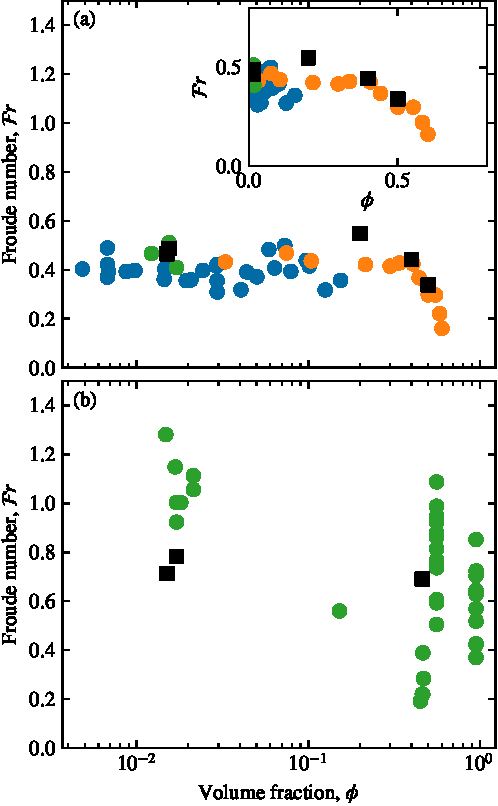
\includegraphics{figure6.pdf}
	\caption{\textbf{Influence of particle volume fraction.} Current Froude number as a function of the initial particle volume fraction for (a) $\alpha \approx 0^\circ$, and (b) $\alpha \approx 45^\circ$. The inset in (a) shows the plot in linear scale.}
	\label{fig:fig6}
\end{figure}
The influence of the parameter $\Phi$ on the Froude number is presented in Figure~\ref{fig:fig6}. The results demonstrate the existence of a critical fraction $\Phi_{c}$ above which the Froude number decreases. This reduction is characterized by an increase particle-particle and particle-fluid interactions which leads in wall friction and a decrease in inertial forces, resulting in a corresponding increase in viscous forces. This results in the decrease of the front velocity and the collapse of the current with the presence of a strong mass fraction gradient near the front.


\subsection*{Acknowledgment}
Sylvain Dauge for the full designing of Setup 2. Hervé Bellot and Brivaël Collin are thanked for experimental support.

\subsection*{Fundings}
ANR PALAGRAM

\bibliographystyle{apalike}
\bibliography{biblio}

\end{document}